\chapter{The Karas Pipeline}
\label{cha:karas-pipeline}

This chapter presents the GPU pipeline proposed by
\cite{karas2019data} (henceforth referred to as the \textit{Karas
  Pipeline} in more detail since the work presented in this report is
directly based off of this seminal work. The chapter concludes by
presenting the limitations of the Karas Pipeline and derives
motivations for a better alternative as presented in the following
chapters (see chapters \ref{cha:pm} and \ref{cha:gcd}).

Karas et al. presents a data processing pipeline to filter timeslices
containing hits from neutrino events from those containing only noise.
The pipeline is able to achieve this filtration by processing the data
in 3 steps, illustrated in Figure \ref{fig:karas-pipeline} and
described in more detail below. Figure \ref{fig:karas-pipeline-data}
provides a visual representation of the various shapes and
arrangements of the data as it passes through the pipeline.

\begin{figure}[h]
  \centering
  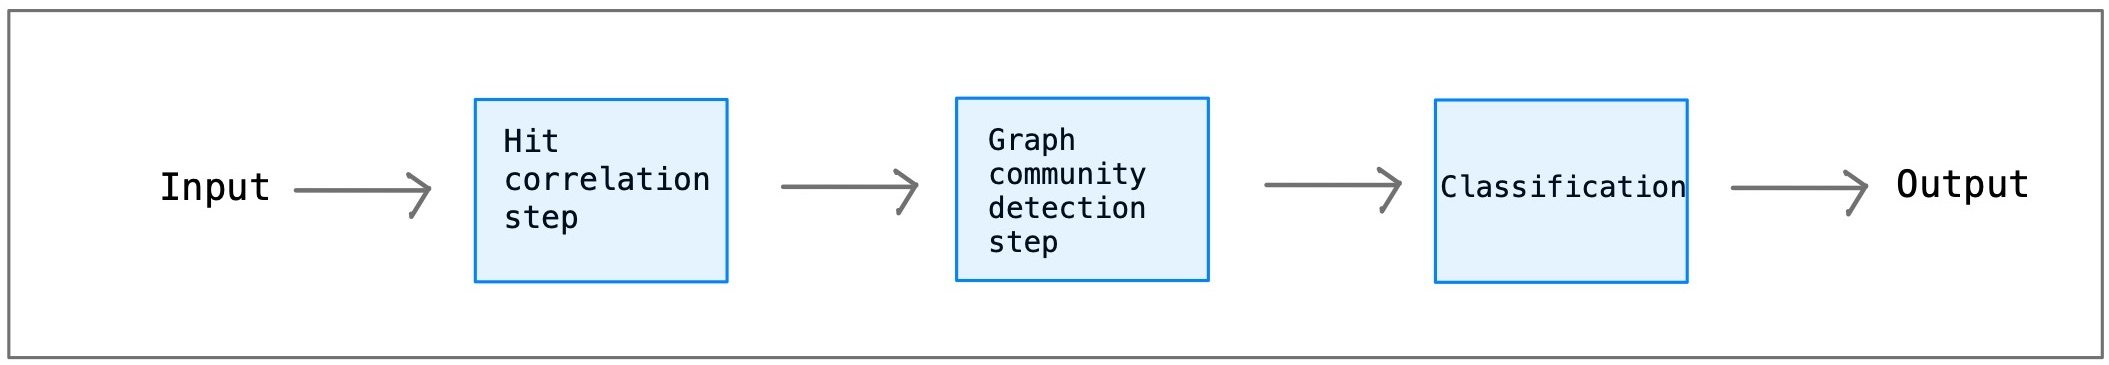
\includegraphics[width=\textwidth]{karas-pipeline.jpg}
  \caption{Overview of Karas Pipeline}
  \label{fig:karas-pipeline}
\end{figure}

\begin{figure}[h]
  \centering
  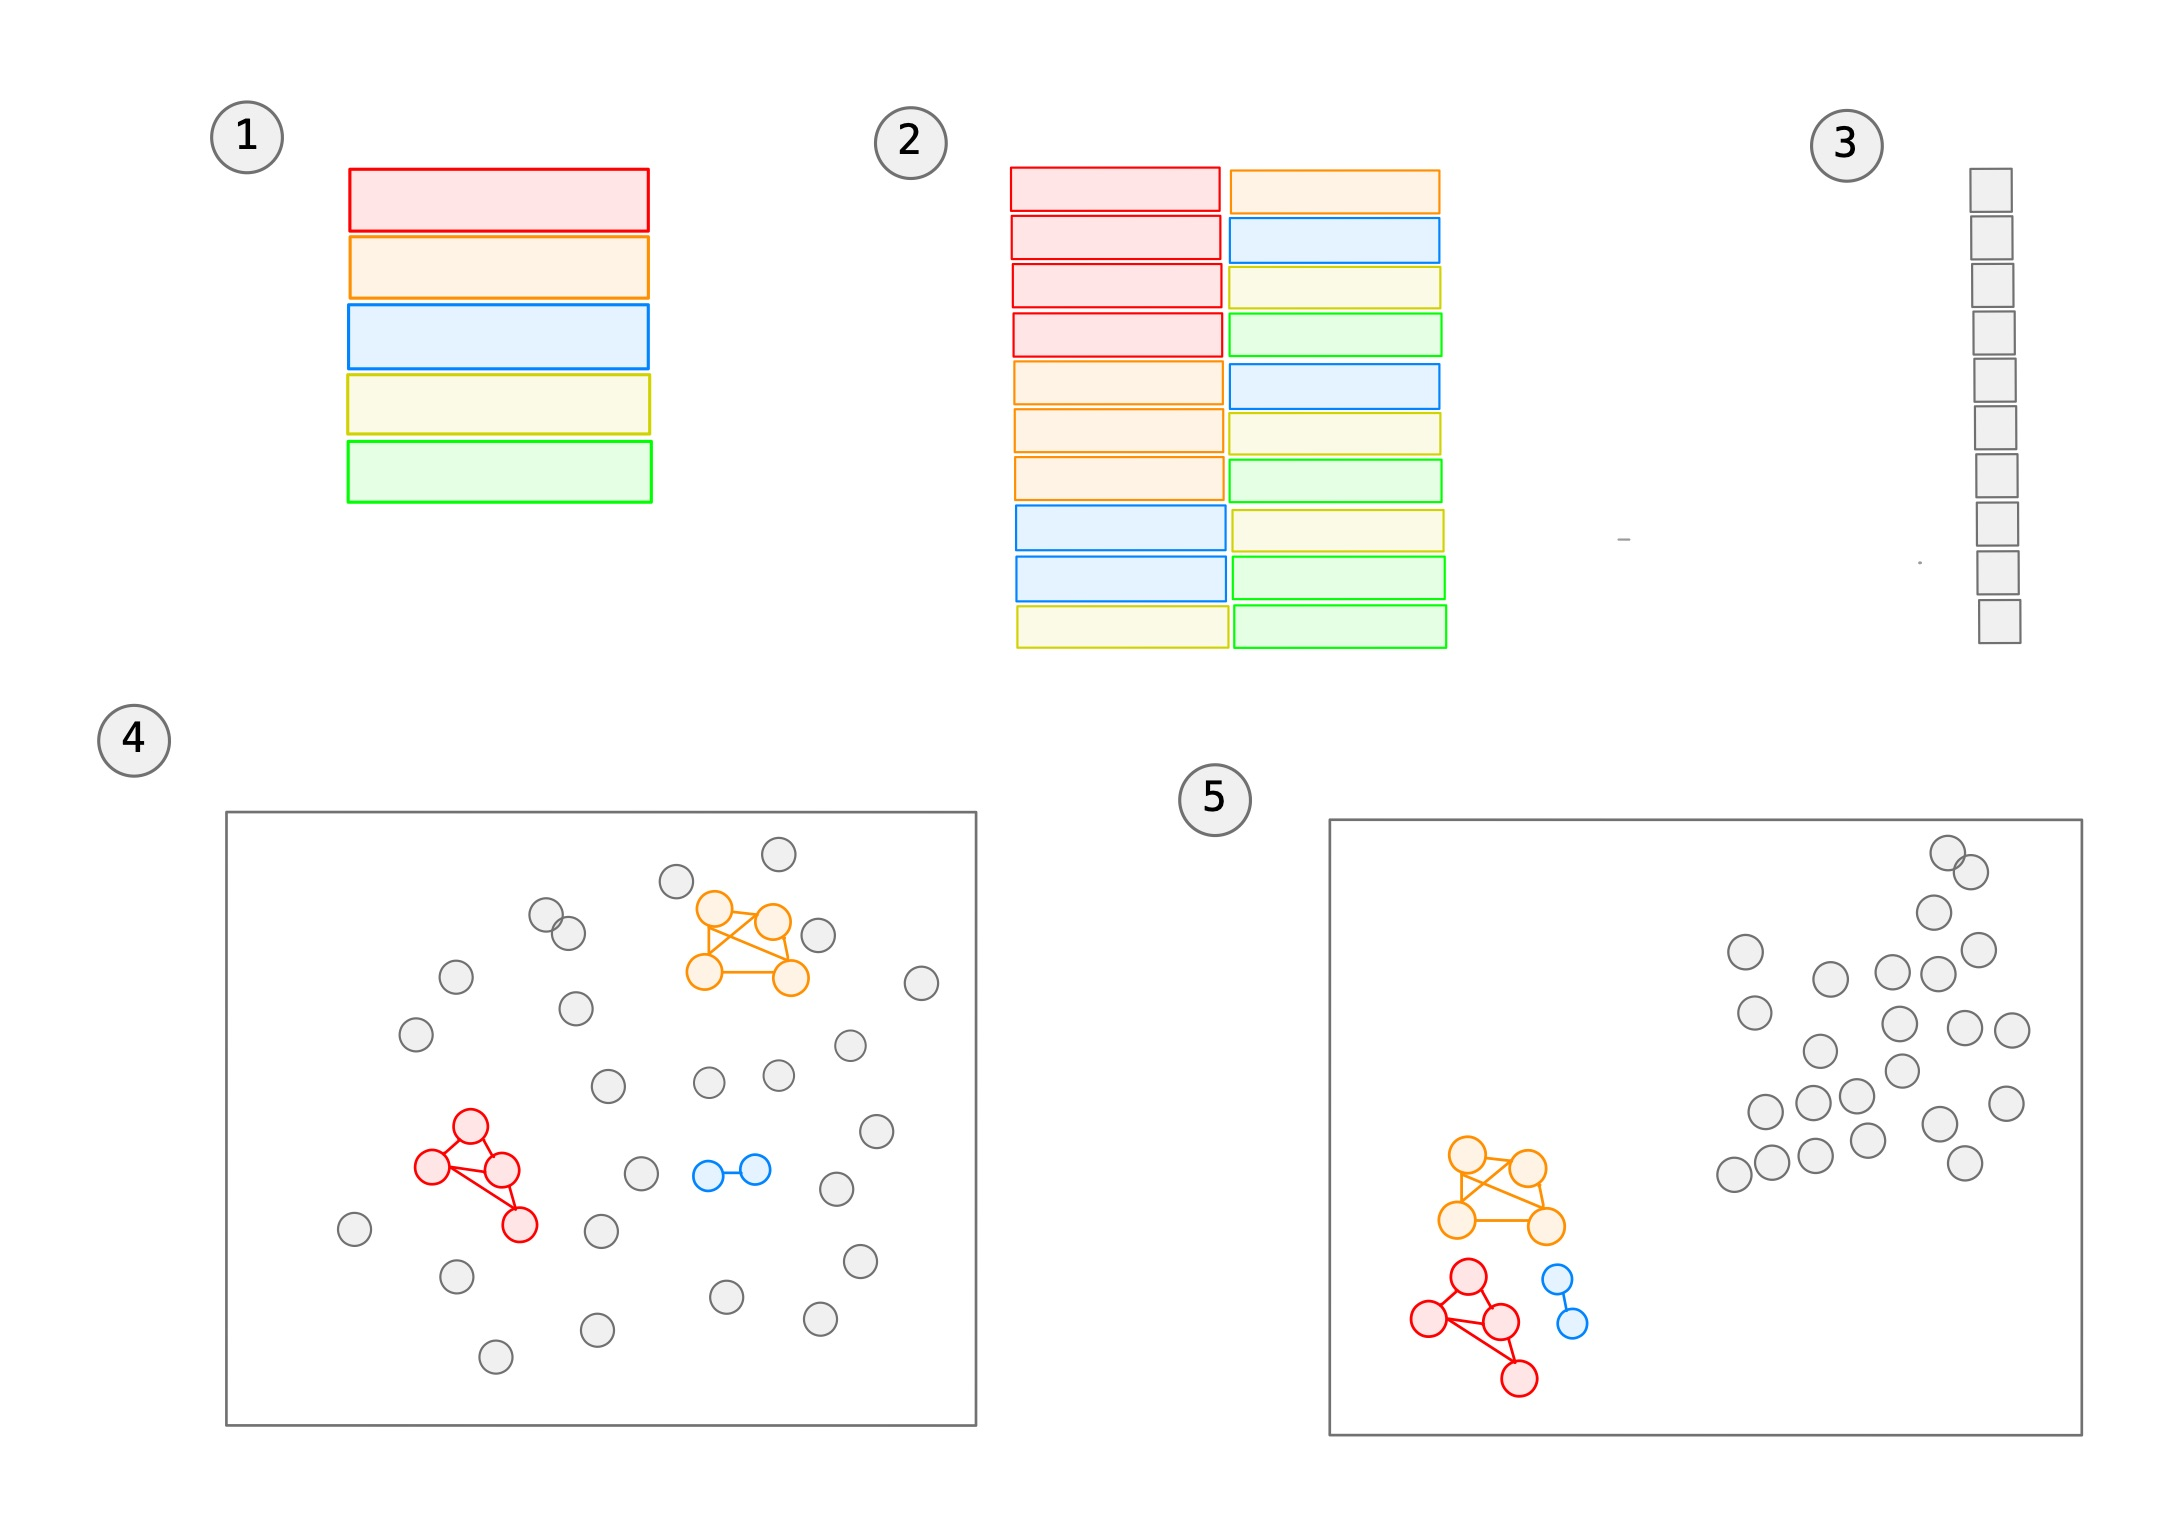
\includegraphics[width=\textwidth]{karas-pipeline-data.jpg}
  \caption{\textbf{(1)}. The main dataset of the project, each row
    representing a hit consisting of the $(x, y, z, t) vector$. Here
    an example set containing 5 hits is shown. \textbf{(2)}. The input
    to the Correlation Step is all unique pairs of hits. \textbf{(3)}.
    The output of the Correlation Step is a vector containing the
    probability that the pairs of hits are related to each other.
    \textbf{(4)}. (1) and (3) are used to construct a graph
    representation of the dataset where event (red, orange and blue)
    and noise (grey) hits are represented as nodes and related nodes
    are connected by an undirected edge carrying as weight the
    probability of being related. \textbf{(5)}. The graph from (4)
    acts as the input to the Graph Community Detection step, the
    output of which is another graph where event and noise nodes are
    grouped together and thus are linearly separable from each other.}
  \label{fig:karas-pipeline-data}
\end{figure}

The first step of The Karas pipeline is the Hit Correlation step. In
this step, pairs of hits (from events and noise) are considered and
the correlation along two axes namely space and time are considered.
Karas et al. proposes \textit{The Pattern Matrix Criterion (PMC)}. The
PMC operates by creating a correlation criterion based on the
probability that a given space and time difference occurs between two
event hits. From domain knowledge, the evaluation is limited to 100m
and 300ns for space and time differences respectively. The algorithm
is evaluated with a dataset containing 130 event hits and 5000 noise
hits and scores in the range of 0.3 - 0.375 is reported for the
recall, precision and F1 metrics and an accuracy of 80\% is achieved.

The second step of the Karas pipeline is the Graph Community Detection
step. The Constant Potts Model (CPM) is used to group event and noise hits
(represented as nodes of a graph) into separate communities (or clusters)
based on the density of connections and the size of the communities. The
output of the PMC is utilized to connect causally related nodes with an
undirected edge and the probability of correlation is assigned as the weight
of the edge. The model is tested using a dataset consisting of 130 event hits
and 5000 noise hits. The model is able to perform exceptionally well and
groups most event hits into a single community and the noise in another. No
performance metrics are reported however.

The third and final step of the pipeline is the Classification step. The two
parameters namely the Probability Threshold (PT) of the PMC and the $\gamma$
of the GCD step are experimented with to determine the optimal thresholds. All
hits above the specified thresholds are classified as event hits the rest are
classified as noise.

\subsection{Limitations of the Karas Pipeline}
\label{sec:karas-pipeline-limitations}

% limitation: edges are only assigned to nodes which are deemed to be related
% by the PMC, since the probability threshold is manually set, some event hits
% may get classified as noise
% limitation: the communities are created by looking at the density of
% connections and size of communities, some really small event communities may
% get overlooked

% step 3: classification step
% - tested with 1,000,000 hits; ~7000 event hits and the rest noise
% - based on output of the GCD step, timeslices with event communities are
%   classified as important and the rest not important
% - experiments with the PT and \gamma parameters are done to determine the
% optimal model
% - communities above the PM and \gamma thresholds are considered to be event
%   hits and the rest noise
% limitation: unable to classify communities of size smaller than 20 hits

The Karas Pipeline is able to identify timeslices with neutrino event
hits more accurately compared to its predecessors such as the L1 and
the L2 filtration. However, the pipeline still has certain limitations
which hinders its performance, thus motivating a need for a better
alternative.

To begin, the space and time difference based on which the PMC
determines if two hits are causally related to one another, is static.
This results in event hits which do not meet these thresholds to be
incorrectly given a low probability of correlation to its sibling
(related) hits.

The performance of the GCD step directly depends on the output of the
PMC since the edges between causally related nodes and the weight it
carries is determined from the PMC. Thus, any limitations of the PMC
cascade down into the GCD and by extension, also into the
classification step.

% the PT is static, this may incorrectly classify event hits as noise

The CPM creates communities by observing the density of connections
and the size of the communities. These thresholds are once again
static which results in small communities being overlooked.

Finally, the classification step also operates on static values of the
PT and $\gamma$ and thus is unable to identify communities of size
smaller than 20 hits.
